\documentclass[a4paper]{article}

\usepackage[utf8]{inputenc}
\usepackage[T1]{fontenc}
\usepackage{textcomp}
\usepackage[english]{babel}
\usepackage{amsmath, amssymb}


%figure support
\usepackage{import}
\usepackage{xifthen}
\pdfminorversion=7
\usepackage{pdfpages}
\usepackage{transparent}
\newcommand{\incfig}[1]{%
	\def\svgwidth{\columnwidth}
	\import{./figures/}{#1.pdf_tex}
}
\graphicspath{ {./figures/} }
\pdfsuppresswarningpagegroup=1

\begin{document}
	\title{Mini-Project 0 Due: 1/14/19}
	\author{Brandon Thompson }
	\maketitle

	\section*{Project Description}
	\begin{itemize}
		\item Install an Ubuntu virtual machine.
		\item Download xv6 from Canvas and transfer it to the virtual machine.
		\item Modify the \verb+ls+ command to print ''Hello''.
	\end{itemize}

	\section*{'rename later'}
	\begin{itemize}
		\item Modify \verb|Makefile| in \verb|xv6/| to include \verb|qemu-system-i386|.
			\begin{figure}[ht!]
				\centering
				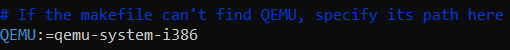
\includegraphics[width=0.8\textwidth]{1}
			\end{figure}
		\item Make a copy of \verb|ls.c| in \verb|xv6/user| with name \verb|hello.c|.
			\begin{figure}[ht!]
				\centering
				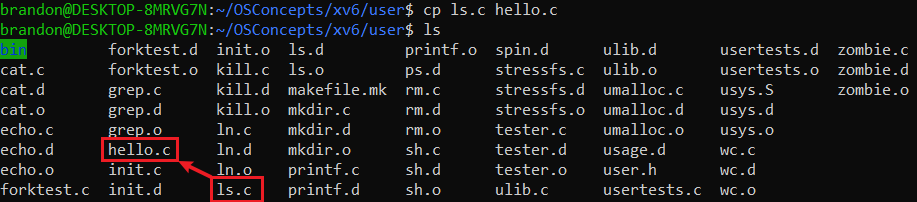
\includegraphics[width=0.8\textwidth]{2}
			\end{figure}
		\item Delete majority of the contents of \verb|hello.c|, leaving include statements
			and main function.
		\item Modify main function to print ''Hello''.
			\begin{figure}[ht!]
				\centering
				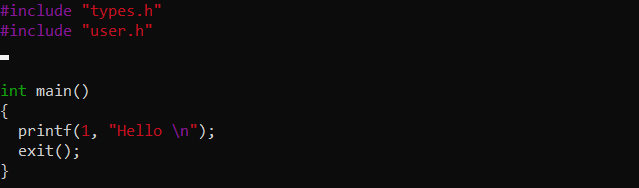
\includegraphics[width=0.8\textwidth]{3}
			\end{figure}
		\item Update the \verb|makefile.mk| file to include hello as a command.
			\begin{figure}[ht!]
				\centering
				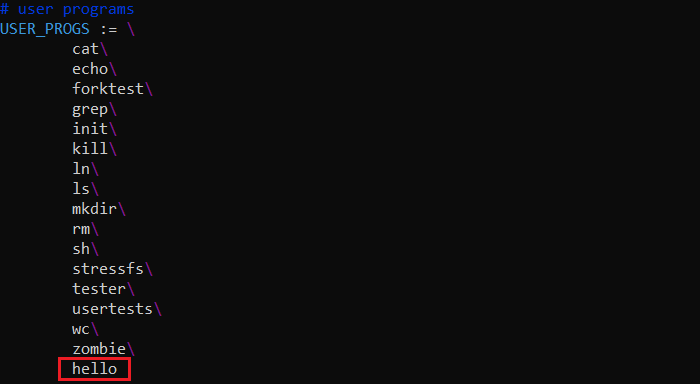
\includegraphics[width=0.8\textwidth]{4}
			\end{figure}
		\item Compile and start xv6 with \verb|make qemu-nox|.
		\item Verify execution of hello command.
			\begin{figure}[ht!]
				\centering
				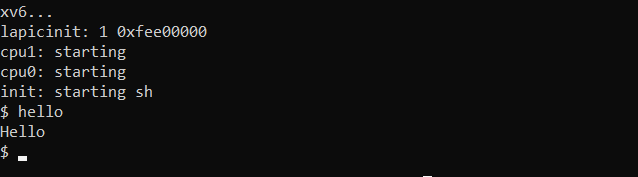
\includegraphics[width=0.8\textwidth]{5}
			\end{figure}
	\end{itemize}
	
\end{document}
